\documentclass{beamer}
\usetheme{Madrid} % Clean theme
\usepackage{listings}
\usepackage{xcolor}
\usepackage{graphicx}

\usepackage{gvv}

% Code listing style
\lstset{
  basicstyle=\ttfamily\footnotesize,
  keywordstyle=\color{blue},
  stringstyle=\color{orange},
  commentstyle=\color{green!60!black},
  breaklines=true,
  frame=single,
  showstringspaces=false
}

\title{MatGeo Assignment - Problem 2.10.55}
\author{EE25BTECH11024}
\institute{IIT Hyderabad}

\begin{document}

% Title slide
\begin{frame}
  \titlepage
\end{frame}

% Problem statement
\begin{frame}{Problem Statement}
The edges of a parallelepiped are of unit length and are parallel to non-coplanar unit vectors $\vec{a}, \vec{b}, \vec{c}$ such that $\vec{a} \cdot \vec{b} = \vec{b} \cdot \vec{c} = \vec{c} \cdot \vec{a} = \frac{1}{2}$. Then, the volume of the parallelepiped is
\begin{enumerate}[label=(\alph*)]
    \item $\dfrac{1}{\sqrt{2}}$
    \item $\dfrac{1}{2\sqrt{2}}$
    \item $\dfrac{\sqrt{5}}{2}$
    \item $\dfrac{1}{\sqrt{3}}$
\end{enumerate}
\end{frame}

% Solution using Rank Criterion (Slide 1)
\begin{frame}{Solution:}
\noindent
\begin{center}
    \begin{tabular}{|c|c|p{5cm}|}
    \hline
    \textbf{Symbol} & \textbf{Value / Definition} & \textbf{Description}  \\
    \hline
    $\vec{a}, \vec{b}, \vec{c}$ & $|\vec{a}|=|\vec{b}|=|\vec{c}|=1$ & Non-coplanar unit vectors for the parallelepiped edges. \\
    \hline
    $\vec{a}\cdot\vec{b}, \vec{b}\cdot\vec{c}, \vec{c}\cdot\vec{a}$ & $\dfrac{1}{2}$ & The dot product between any pair of the vectors. \\
    \hline
    $A$ & $\myvec{ \vec{a} & \vec{b} & \vec{c} }$ & A $3\times3$ matrix with the edge vectors as its columns. \\
    \hline
    $V$ & $|\det(A)|$ & The volume of the parallelepiped (the value to be found). \\
    \hline
    \end{tabular}
\end{center}
\noindent
\end{frame}

\begin{frame}{Solution: }
Using Gram matrix,  
\begin{align}
    G = A^\top A = 
    \myvec{\vec{a} & \vec{b} & \vec{c}}^\top
    \myvec{ \vec{a} & \vec{b} & \vec{c} }
    = \myvec{\vec{a}\cdot\vec{a} & \vec{a}\cdot\vec{b} & \vec{a}\cdot\vec{c} \\
             \vec{b}\cdot\vec{a} & \vec{b}\cdot\vec{b} & \vec{b}\cdot\vec{c} \\
             \vec{c}\cdot\vec{a} & \vec{c}\cdot\vec{b} & \vec{c}\cdot\vec{c}}
\end{align}

Substituting the given values into the Gram matrix:
\begin{align}
    G = \myvec{1 & 1/2 & 1/2 \\ 1/2 & 1 & 1/2 \\ 1/2 & 1/2 & 1}
\end{align}
The determinant of the Gram matrix is related to the determinant of $A$ by:
\begin{align}
    \det(G) = 
    \det(A^\top A) = (\det(A))^2 = V^2
\end{align}
Therefore, the volume is $V = \sqrt{\det(G)}$.
\end{frame}

\begin{frame}{Solution: }
Calculating determinant of G we get,
\begin{align}
    \det(G) & \\
    =\det\myvec{
1 & 1/2 & 1/2 \\
1/2 & 1 & 1/2 \\
1/2 & 1/2 & 1
}
& \xrightarrow[R_3 \to R_3 - \frac{1}{2}R_1]{R_2 \to R_2 - \frac{1}{2}R_1}
\det\myvec{
1 & 1/2 & 1/2 \\
0 & 3/4 & 1/4 \\
0 & 1/4 & 3/4
}
\\[2em] % Adds extra vertical space
= \det\myvec{
1 & 1/2 & 1/2 \\
0 & 3/4 & 1/4 \\
0 & 1/4 & 3/4
}
& \xrightarrow{R_3 \to R_3 - \frac{1}{3}R_2}
\det\myvec{
1 & 1/2 & 1/2 \\
0 & 3/4 & 1/4 \\
0 & 0 & 2/3
} \\
 = \frac{1}{2} = \det(G)
\end{align}
Therefore, volume $V$ is,
\begin{align}
    V = \sqrt{\det(G)}  = \frac{1}{\sqrt{2}}
\end{align}
\end{frame}

\begin{frame}{Final Answer}
Thus, the volume of the parallelepiped is $\dfrac{1}{\sqrt{2}}$, which corresponds to option (a).

See Figure~\ref{fig:3DVectors}.  
\end{frame}

\begin{frame}{Figure}
    \begin{figure}[h!]
    \centering
    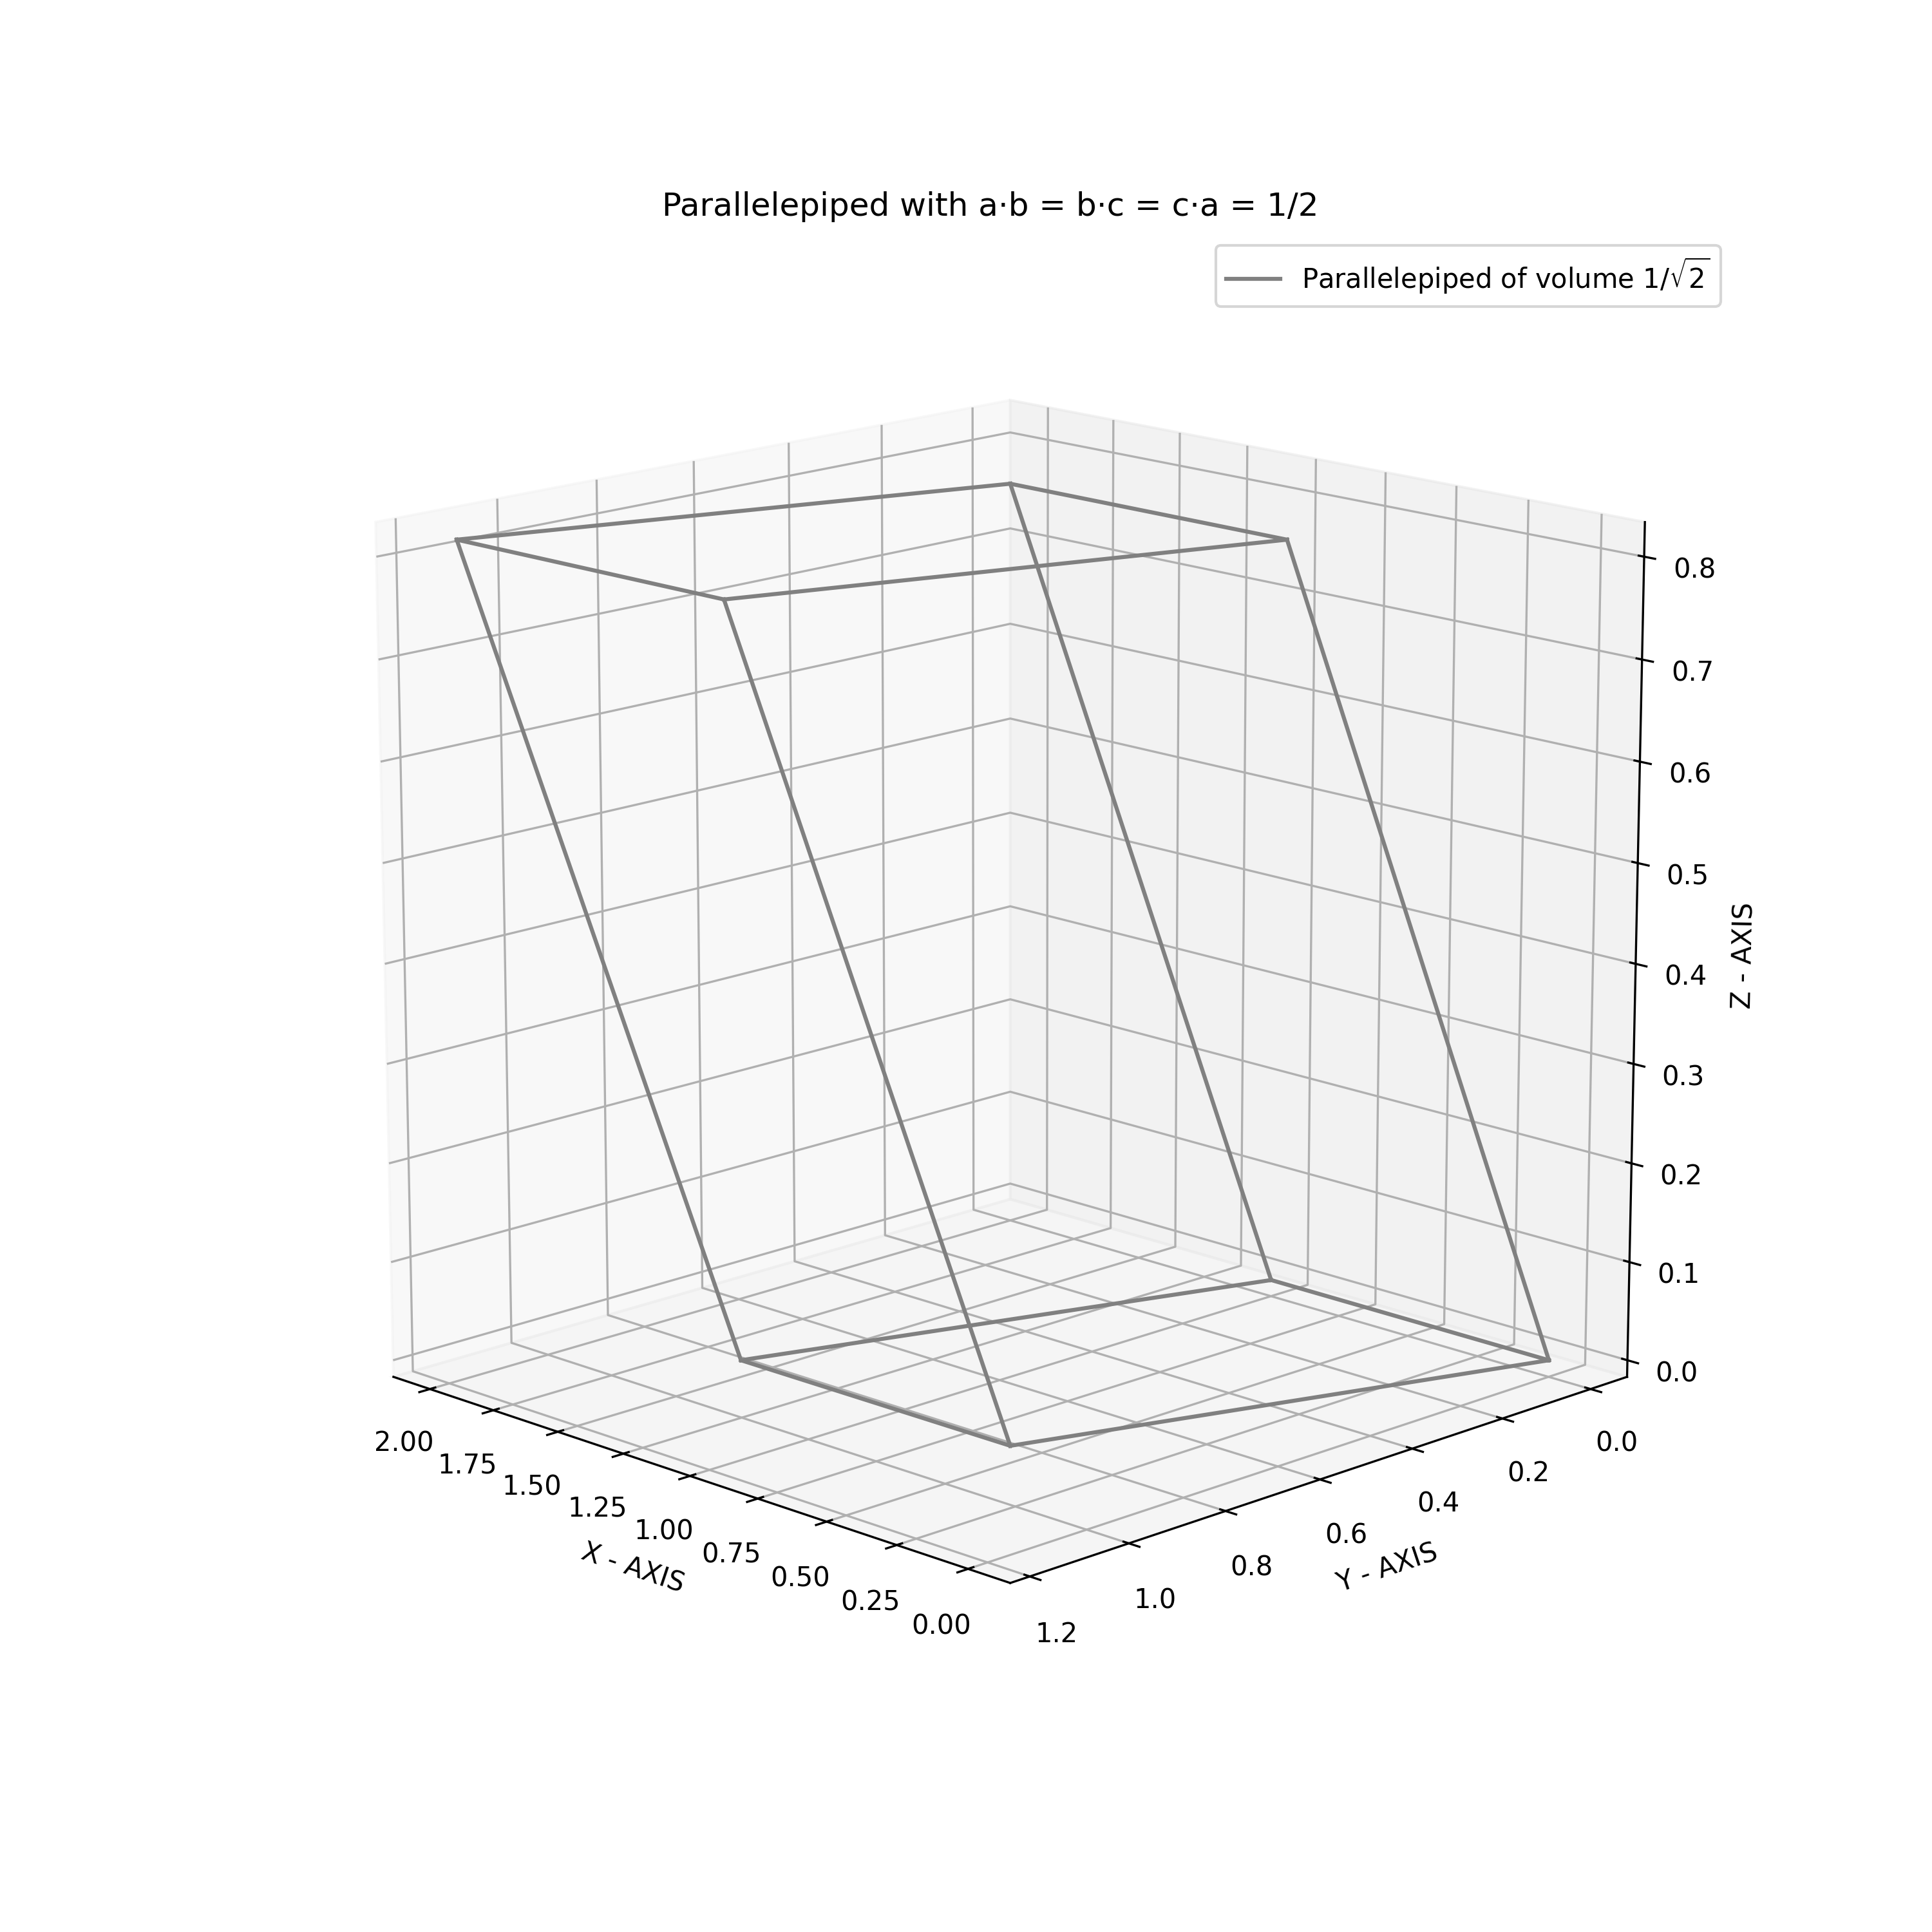
\includegraphics[width=0.7\linewidth]{figs/fig.png}
    \caption{}
    \label{fig:3DVectors}
\end{figure}
\end{frame}

% Python code 1
\begin{frame}[fragile]{Python Code: plot.py (Native)}
\begin{lstlisting}[language=Python]
import numpy as np
import matplotlib.pyplot as plt
from mpl_toolkits.mplot3d import Axes3D

a = np.array([1, 0, 0])
b = np.array([0.5, np.sqrt(3)/2, 0])
c = np.array([0.5, 1/(2*np.sqrt(3)), np.sqrt(2/3)])

# Vertices of parallelepiped
p1 = np.array([0,0,0])
p2 = a
p3 = b
p4 = c
p5 = a+b
p6 = b+c
p7 = c+a
p8 = a+b+c
\end{lstlisting}
\end{frame}


\begin{frame}[fragile]{Python Code (Native Implementation – plot.py)}
\begin{lstlisting}[language=Python]
fig = plt.figure(figsize=(10,10))
ax = fig.add_subplot(111, projection='3d')

# Bottom face
ax.plot([p1[0], p2[0]], [p1[1], p2[1]], [p1[2], p2[2]], 'grey')
ax.plot([p1[0], p3[0]], [p1[1], p3[1]], [p1[2], p3[2]], 'grey')
ax.plot([p2[0], p5[0]], [p2[1], p5[1]], [p2[2], p5[2]], 'grey')
ax.plot([p3[0], p5[0]], [p3[1], p5[1]], [p3[2], p5[2]], 'grey')

# Top face
ax.plot([p4[0], p7[0]], [p4[1], p7[1]], [p4[2], p7[2]], 'grey')
ax.plot([p4[0], p6[0]], [p4[1], p6[1]], [p4[2], p6[2]], 'grey')
ax.plot([p7[0], p8[0]], [p7[1], p8[1]], [p7[2], p8[2]], 'grey')
ax.plot([p6[0], p8[0]], [p6[1], p8[1]], [p6[2], p8[2]], 'grey')

# Vertical edges
ax.plot([p1[0], p4[0]], [p1[1], p4[1]], [p1[2], p4[2]], 'grey')
ax.plot([p2[0], p7[0]], [p2[1], p7[1]], [p2[2], p7[2]], 'grey')
ax.plot([p3[0], p6[0]], [p3[1], p6[1]], [p3[2], p6[2]], 'grey')
ax.plot([p5[0], p8[0]], [p5[1], p8[1]], [p5[2], p8[2]], 'grey')
\end{lstlisting}
\end{frame}

\begin{frame}[fragile]{Python Code (Native Implementation – plot.py)}
\begin{lstlisting}[language=Python]
ax.plot([], [], [], 'grey', label=r"Parallelepiped of volume $1/\sqrt{2}$")

ax.set_xlabel("X - AXIS")
ax.set_ylabel("Y - AXIS")
ax.set_zlabel("Z - AXIS")
ax.set_title("Parallelepiped with a·b = b·c = c·a = 1/2")
ax.legend()
ax.set_box_aspect([1,1,1])
ax.view_init(elev=15, azim=135)
plt.savefig("parallelepiped.png", dpi=300)
plt.show()
\end{lstlisting}
\end{frame}

\begin{frame}[fragile]{C Code (Shared Library – findparalellepipedvol.c)}
\begin{lstlisting}[language=C]
#include <stdio.h>
#include <math.h>

double determinant3x3(double m[3][3]) {
    return m[0][0]*(m[1][1]*m[2][2] - m[1][2]*m[2][1])
         - m[0][1]*(m[1][0]*m[2][2] - m[1][2]*m[2][0])
         + m[0][2]*(m[1][0]*m[2][1] - m[1][1]*m[2][0]);
}

double parallelepiped_volume(double *a, double *b, double *c) {
    double m[3][3] = {
        {a[0], b[0], c[0]},
        {a[1], b[1], c[1]},
        {a[2], b[2], c[2]}
    };
    double det = determinant3x3(m);
    return fabs(det); // absolute value = volume
}
\end{lstlisting}
\end{frame}

% Python code 2
\begin{frame}[fragile]{Python Code: call.py (C + Python)}
\begin{lstlisting}[language=Python]
import ctypes
import numpy as np
import matplotlib.pyplot as plt
from mpl_toolkits.mplot3d import Axes3D

lib = ctypes.CDLL("./find_parallelepiped_vol.so")
lib.parallelepiped_volume.argtypes = [
    ctypes.POINTER(ctypes.c_double),
    ctypes.POINTER(ctypes.c_double),
    ctypes.POINTER(ctypes.c_double)
]
lib.parallelepiped_volume.restype = ctypes.c_double

a = np.array([1,0,0], dtype=np.float64)
b = np.array([0.5, np.sqrt(3)/2, 0], dtype=np.double)
c = np.array([0.5, 1/np.sqrt(12), np.sqrt(2/3)], dtype=np.double)

a_ptr = a.ctypes.data_as(ctypes.POINTER(ctypes.c_double))
b_ptr = b.ctypes.data_as(ctypes.POINTER(ctypes.c_double))
c_ptr = c.ctypes.data_as(ctypes.POINTER(ctypes.c_double))
\end{lstlisting}
\end{frame}

\begin{frame}[fragile]{Python Code (C Integrated – call.py)
}
\begin{lstlisting}[language=Python]
volume = lib.parallelepiped_volume(a_ptr, b_ptr, c_ptr)

O = np.array([0,0,0])
points = np.array([
    O, a, b, c, a+b, b+c, c+a, a+b+c
])

edges = [(0,1),(0,2),(0,3),
         (1,4),(1,6),
         (2,4),(2,5),
         (3,5),(3,6),
         (4,7),(5,7),(6,7)]

fig = plt.figure(figsize=(8,8))
ax = fig.add_subplot(111, projection='3d')

for i,j in edges:
    ax.plot([points[i,0],points[j,0]],
            [points[i,1],points[j,1]],
            [points[i,2],points[j,2]], 'grey')
            
\end{lstlisting}
\end{frame}

\begin{frame}[fragile]{Python Code (C Integrated – call.py)
}
\begin{lstlisting}[language=Python]
ax.plot([], [], [], color='grey', linestyle='--',
        label=fr"Parallelepiped of volume {volume:.3f}")
ax.set_xlabel("X - AXIS")
ax.set_ylabel("Y - AXIS")
ax.set_zlabel("Z - AXIS")
ax.set_title("Parallelepiped with a·b = b·c = c·a = 1/2")
ax.legend()                                          ax.set_box_aspect([1,1,1])
ax.view_init(elev=15, azim=135)                      
plt.savefig("parallelepiped_volume.png", dpi=300)
plt.show()
\end{lstlisting}
\end{frame}


\end{document}



